% !TeX spellcheck = en_GB
\documentclass[10pt]{beamer}
\usetheme{CambridgeUS}
%\usetheme{Boadilla}
\definecolor{myred}{RGB}{163,0,0}
%\usecolortheme[named=blue]{structure}
\usecolortheme{dove}
\usefonttheme[]{professionalfonts}
\usepackage[english]{babel}
\usepackage{amsmath,amsfonts,amssymb}
\usepackage{xcolor}
\usepackage{bm}
\usepackage{gensymb}
\usepackage{verbatim} 
\usepackage{paratype}
\usepackage{mathpazo}
\usepackage{listings}
\lstset{language=Python}

% Number theorem environments
\setbeamertemplate{theorem}[ams style]
\setbeamertemplate{theorems}[numbered]

% Reset theorem-like environments so that each is numbered separately
\usepackage{etoolbox}
\undef{\definition}
\theoremstyle{definition}
\newtheorem{definition}{\translate{Definition}}
\newtheorem{Fact}{\translate{Fact}}

% Change colours for theorem-like environments
\definecolor{mygreen1}{RGB}{0,96,0}
\definecolor{mygreen2}{RGB}{229,239,229}
\setbeamercolor{block title}{fg=white,bg=mygreen1}
\setbeamercolor{block body}{fg=black,bg=mygreen2}



\alt<presentation>
{\lstset{%
  basicstyle=\footnotesize\ttfamily,
  commentstyle=\slshape\color{green!50!black},
  frame = single,  
  keywordstyle=\bfseries\color{blue!50!black},
  identifierstyle=\color{blue},
  stringstyle=\color{orange},
  %escapechar=\#,
  showstringspaces = false,
  showtabs = false,
  tabsize = 2,
  emphstyle=\color{red}}
}
{
  \lstset{%
    basicstyle=\ttfamily,
    keywordstyle=\bfseries,
    commentstyle=\itshape,
    escapechar=\#,
    showtabs = false,
	tabsize = 2,
    emphstyle=\bfseries\color{red}
  }
} 

\title{R401: Statistical and Mathematical Foundations}
\subtitle{Lecture 14: Unconstrained Optimization. Static Optimization with Equality Constraints. Lagrange Multipliers}
\author{Andrey Vassilev}

\date{2016/2017} 

\begin{document}
\maketitle

\begin{frame}[fragile]
\frametitle{General Principles and Caveats for the Optimization Module}
\begin{itemize}
\item Emphasis on practicality over rigour
\item Consequently, algorithmic approach and ``recipes'' rather than proofs
\item Also, existence and relevant properties of various objects are often implicitly assumed
\item Pathologies and mathematical peculiarities discussed only in special cases
\end{itemize}
\end{frame}

\begin{frame}[fragile]
\frametitle{Lecture Contents}
\tableofcontents
\end{frame}




\section{Warm-up: Basic Unconstrained Optimization in $ \mathbb{R}^1 $}\label{sec:R1}

\begin{frame}[fragile]
\frametitle{Warm-up: Basic Unconstrained Optimization in $ \mathbb{R}^1 $}

\begin{Fact}
For a function $ f: \mathbb{R} \rightarrow \mathbb{R} $ differentiable at a point $ x $, a necessary condition for a local extreme point (i.e. a maximum or a minimum) at $ x $ is \[ f'(x) = 0. \]
\end{Fact}
\bigskip

\begin{example} %{Example}
If $ f(x) = ax^2 + bx + c $, then $ f'(x) = 2ax + b $ and the condition $ f'(x)=0 $ yields the familiar $ x=-\frac{b}{2a} $ (recall your high-school days). Depending on the sign of $ a $, this is a maximum or a minimum (What is the relationship?).
\end{example}\bigskip

\begin{example} %{Example}
If $ f(x) = x^3 $, then $ f'(x)=3x^2 $ and $ f'(x)=0 \Rightarrow x=0$.

Does the function attain a maximum or a minimum at $ x=0 $?
\end{example}
\end{frame}

\begin{frame}[fragile]
\frametitle{Warm-up: Basic Unconstrained Optimization in $ \mathbb{R}^1 $}
\begin{figure}
\centering
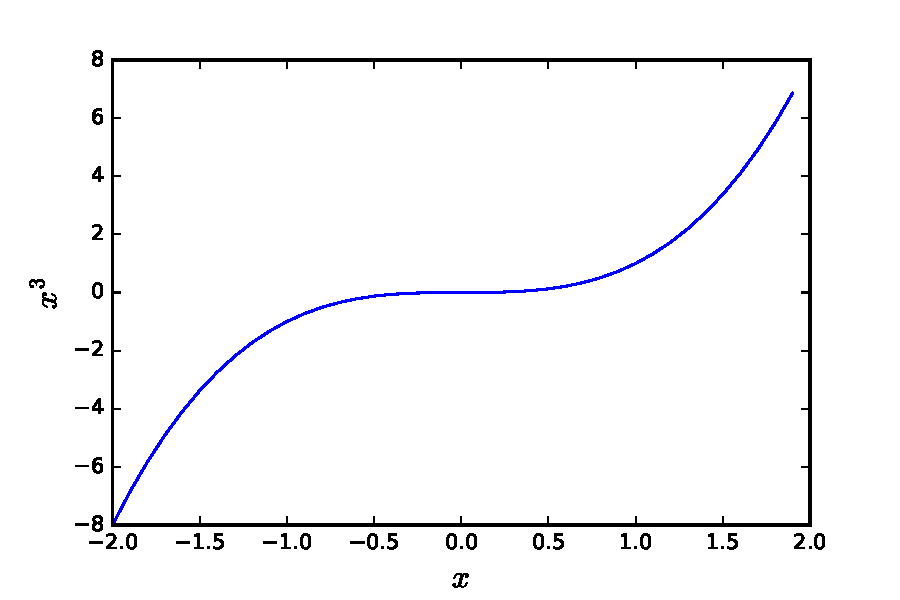
\includegraphics[width=0.9\linewidth]{cubicfun}
\label{fig:cubicfun}
\end{figure}
\end{frame}

\begin{frame}[fragile]
\frametitle{Warm-up: Basic Unconstrained Optimization in $ \mathbb{R}^1 $}
\addtocounter{theorem}{-1}
\begin{example}[cont.]
The answer is ``neither''! The point $ x=0 $ is not a local extreme point of $ f(x)=x^3 $.\medskip

This illustrates the pitfalls of using necessary conditions -- they supply only candidates that need to be checked further.
\end{example}

The above examples generalize in the following manner:
\begin{Fact}
Let a function $ f $ be $ n $ times differentiable at a point $ x $ and 
\[ f'(x)=f''(x)=\ldots=f^{(n-1)}(x)=0,\qquad f^{(n)}\neq 0. \] \vskip -5pt
\begin{enumerate}
\item If $ n $ is odd, the point $ x $ is not an extreme point of $ f(x) $.
\item If $ n $ is even and $ f^{(n)}(x)>0 $, the point $ x $ is a minimum.
\item If $ n $ is even and $ f^{(n)}(x)<0 $, the point $ x $ is a maximum.
\end{enumerate}
\end{Fact}
\end{frame}

\section{Unconstrained Optimization in $ \mathbb{R}^n $}\label{sec:Rn}

\begin{frame}[fragile]
\frametitle{Unconstrained Optimization in $ \mathbb{R}^n $}
\framesubtitle{Necessary conditions}
\begin{Fact}
For a function $ f: S \rightarrow \mathbb{R},~ S \subseteq \mathbb{R}^n$, differentiable at an interior point $ \mathbf{x} $, a necessary condition for $ \mathbf{x} $ to be a local extreme point is \[ f'(\mathbf{x}) = \mathbf{0}, \]
where \[ \mathbf{x} = \left( \begin{array}{c}
x_1 \\
x_2\\
\vdots \\
x_n
\end{array}\right),~\mathbf{0} = \left( \begin{array}{c}
0 \\
0 \\
\vdots \\
0
\end{array}\right)\text{ and }  f'(\mathbf{x}) = \left( \begin{array}{c}
\dfrac{\partial f(x_1,\ldots,x_n)}{\partial x_1}\\
\vdots \\
\dfrac{\partial f(x_1,\ldots,x_n)}{\partial x_n}
\end{array}\right) \]
\end{Fact}
\end{frame}

\begin{frame}[fragile]
\frametitle{Unconstrained Optimization in $ \mathbb{R}^n $}
\begin{example}
\[ f(x,y) = x^2 +2y^2-3x+xy \]
\[ \frac{\partial f}{\partial x} = 2x-3+y=0\quad \Rightarrow \quad x=\frac{3-y}{2} \]
\[ \frac{\partial f}{\partial y} = 4y+x = 0\quad \Rightarrow \quad y = -\frac{x}{4}\]
\[ x=\frac{12}{7},~y=-\frac{3}{7} \]
\end{example}
\end{frame}


\end{document}